\documentclass[UTF8]{ctexart}


\usepackage{float}

\usepackage{tikz,mathpazo}
\usetikzlibrary{shapes.geometric, arrows}
\usetikzlibrary{calc}


\usepackage{listings}
%插入代码的配置
\definecolor{CPPLight}  {HTML} {686868}
\definecolor{CPPSteel}  {HTML} {888888}
\definecolor{CPPDark}   {HTML} {262626}
\definecolor{CPPBlue}   {HTML} {4172A3}
\definecolor{CPPGreen}  {HTML} {487818}
\definecolor{CPPBrown}  {HTML} {A07040}
\definecolor{CPPRed}    {HTML} {AD4D3A}
\definecolor{CPPViolet} {HTML} {7040A0}
\definecolor{CPPGray}  {HTML} {B8B8B8}
\lstset{
	language=Python,                                     % 设置语言
    columns=fixed,    
    breaklines = true,   
    basicstyle=\small ,
    numbers=left,                                        % 在左侧显示行号
    %frame=none,                                          % 不显示背景边框
    backgroundcolor=\color[RGB]{245,245,244},            % 设定背景颜色
    keywordstyle=\color[RGB]{40,40,255},                 % 设定关键字颜色
    numberstyle=\tiny\color{darkgray},           % 设定行号格式
    %commentstyle=\it\color[RGB]{0,96,96},                % 设置代码注释的格式
    stringstyle=\rmfamily\slshape\color[RGB]{128,0,0},   % 设置字符串格式
    showstringspaces=false,                              % 不显示字符串中的空格                           
    %morekeywords={True,alignas,continute,friend,register,true,alignof,decltype,goto,
    %reinterpret_cast,try,asm,defult,if,return,typedef,auto,delete,inline,short,
    %typeid,bool,do,int,signed,typename,break,double,long,sizeof,union,case,
    %dynamic_cast,mutable,static,unsigned,catch,else,namespace,static_assert,using,
    %char,enum,new,static_cast,virtual,char16_t,char32_t,explict,noexcept,struct,
    %void,export,nullptr,switch,volatile,class,extern,operator,template,wchar_t,
    %const,false,private,this,while,constexpr,float,protected,thread_local,
    %const_cast,for,public,throw,std,rand},
    emph={access,and,break,class,continue,def,del,elif ,else,%
	except,exec,finally,for,from,global,if,import,in,i s,%
	lambda,not,or,pass,print,raise,return,try,while},
    emphstyle=\color{CPPViolet}, 
    emph={[2]True, False, None, self},
	emphstyle=[2]\color{green},
	emph={[3]from, import, as},
	emphstyle=[3]\color{blue},
	upquote=true,
	morecomment=[s]{"""}{"""},
	commentstyle=\color{orange}\slshape,
	emph={[4]1, 2, 3, 4, 5, 6, 7, 8, 9, 0},
	emphstyle=[4]\color{red},
	emph={[5]numpy, np, plt},
	emphstyle=[5]\color{red},
	literate=*{:}{{\textcolor{blue}:}}{1}%
	{=}{{\textcolor{blue}=}}{1}%
	{-}{{\textcolor{blue}-}}{1}%
	{+}{{\textcolor{blue}+}}{1}%
	{*}{{\textcolor{blue}*}}{1}%
	{!}{{\textcolor{blue}!}}{1}%
	{(}{{\textcolor{blue}(}}{1}%
	{)}{{\textcolor{blue})}}{1}%
	{[}{{\textcolor{blue}[}}{1}%
	{]}{{\textcolor{blue}]}}{1}%
	{<}{{\textcolor{blue}<}}{1}%
	{>}{{\textcolor{blue}>}}{1},%
	framexleftmargin=0.1mm, framextopmargin=0.1mm, frame=shadowbox, rulesepcolor=\color{black},
}



\usepackage{geometry}
\geometry{left=2cm, right=2cm, top=1.2cm, bottom=1.2cm}

%得到引用的标题内容
\usepackage{nameref} 

%添加首行缩进,两个字符
\usepackage{indentfirst}
\setlength{\parindent}{2em}

%多行公式一个编号
\usepackage{amsmath}

%文献引用,标准类型为plain
%\usepackage[hyperref=true,backend=biber,sorting=none,backref=true]{biblatex}
%\addbibresource{ref.bib}
\bibliographystyle{plain}
\usepackage{cite}

\pagestyle{plain}


\usepackage{graphicx}

%超链接
\usepackage[linkcolor=yellow,citecolor=red,backref=page]{hyperref}
\hypersetup{
bookmarks=true,
colorlinks=true,
linkcolor=black
}

%引入了一些改进的数学环境,如align
\usepackage{amsmath}

\title{数据结构:祖玛}
\author{姓名:鲁国锐 \protect\newline
\and 学号:17020021031 \\
\and 专业:电子信息科学与技术}


\begin{document}
	\maketitle
	\renewcommand{\contentsname}{Contents}
	\tableofcontents
	\newpage
	
	\hypersetup{
	bookmarks=true,
	colorlinks=true,
	linkcolor=red,
	urlcolor=blue
	}
	\section{问题分析}
	\subsection{题目描述}
	\indent 祖玛是一款曾经风靡全球的游戏,其玩法是:在一条轨道上初始排列着若干个彩色珠子,其中任意三个相邻的珠子不会完全同色。此后,你可以发射珠子到轨道上并加入原有序列中。一旦有三个或更多同色的珠子变成相邻,它们就会立即消失。这类消除现象可能会连锁式发生,其间你将暂时不能发射珠子。

\indent 开发商最近准备为玩家写一个游戏过程的回放工具。他们已经在游戏内完成了过程记录的功能,而回放功能的实现则委托你来完成。

\indent 游戏过程的记录中,首先是轨道上初始的珠子序列,然后是玩家接下来所做的一系列操作。你的任务是,在各次操作之后及时计算出新的珠子序列。
	\subsubsection{输入}
	\indent 第一行是一个由大写字母$’A’~’Z’$组成的字符串,表示轨道上初始的珠子序列,不同的字母表示不同的颜色。

\indent 第二行是一个数字$n$,表示整个回放过程共有$n$次操作。

\indent 接下来的$n$行依次对应于各次操作。每次操作由一个数字$k$和一个大写字母$\sum$描述,以空格分隔。其中,$\sum$为新珠子的颜色。若插入前共有$m$颗珠子,则$k\in[0, m]$表示新珠子嵌入之后(尚未发生消除之前)在轨道上的位序。
	\subsubsection{输出}
	\indent 输出共$n$行,依次给出各次操作(及可能随即发生的消除现象)之后轨道上的珠子序列。

\indent 如果轨道上已没有珠子,则以“$-$”表示。
	\subsubsection{样例}
	\begin{itemize}
	\item 输入
		\begin{itemize}
			\item[ ]ACCBA
			\item[ ]5
			\item[ ]1 B
			\item[ ]0 A
			\item[ ]2 B
			\item[ ]4 C
			\item[ ]0 A
		\end{itemize}
	\item 输出
		\begin{itemize}
			\item[ ]ABCCBA
			\item[ ]AABCCBA
			\item[ ]AABBCCBA
			\item[ ]-
			\item[ ]A	
		\end{itemize}
	\end{itemize}
	
	\subsection{问题分析}
	\indent 根据题目,我们需要解决的问题有:
	\begin{itemize}
	\item[ ] 
	\begin{enumerate}
	\item 如何在插入后找出字符串中三个以上连续字符的位置;
	\item 如何在进行消除后找出字符串中三个以上连续字符的位置;
	\end{enumerate}
	\end{itemize}	
	
	\indent 至于消除的问题可以直接用模板库的函数来解决,所以不在我们要考虑的范围之内。	
	
	
	\section{解决方案}
	\indent 首先这道题需要注意的一点是,\textbf{给定的输入中可能有三个以上连续重复的字符},但根据以往玩游戏的经验,它并不会自动消除,而是需要人为地往里面再添加一个相同字符。所以我们不能每次都对整个字符串进行遍历。事实上,我们也不需要对整个字符串遍历,因为每次可能会出现消除的地方只会是插入后的位置以及消除后的“接口”位置。再进一步考虑,由于消除后后面的元素会向前填补,所以插入位置和消除后的“接口”处可以用同一个下标来表示。所以我们只用反复地考查插入位置附近是否有三个及以上连续相同字符并在符合条件的情况下进行消除。
	
	\indent 由此我们引出了解决本题时需要实现的两个函数:一个是$find$函数,用于考察插入位置附近是否有连续相同字符,返回该字符串的终止位置;一个是$ablat$,用于在符合条件时对find函数找出的字符串进行消除,并返回找出的字符串是否符合条件以确定是否需要再次调用$find$函数进行考察。
	
	\indent 首先我们来看一看$find$函数。为了实现其功能,我们需要对其传入参数插入位置的下标$start$以及目标字符串$balls$。我们再定义两个变量$left$和$right$,分别用来表示连续相同字符序列的起始下标和\textbf{终止下标的下一位}。我们先从$start$开始向左遍历,如果前一个元素等于当前元素,则令$left$减一;再从$start$开始向右遍历,如果下一个元素等于当前元素,则令$right$加一。注意不论是向左还是向右遍历,都不能超出字符串边界。另外还有一个小问题,我们调用$find$函数是为了找出满足条件的子序列的两头,我们可以直接返回$right$来输出末尾的下标,但起始的怎么办?如果是用一个数组来存放两个下标未免太不划算,所以这里我们在传参时直接传入$start$的引用,并在函数结束前把$left$的值赋给$start$即可。
	
	\indent 接下来我们再来看看$ablat$函数。为了实现其功能,我们需要传入起始下标$start$、终止下标$end$以及目标字符串$balls$。我们在定义一个变量$flag$,并令:
	\begin{align}
	flag = ((end - start) \geq 3) \label{flag}
	\end{align}
	
	\indent 公式\ref{flag}的目的是用来判断$find$函数找出的字符串是否满足条件。如果是,则进行消除。最后再返回$flag$给主函数判断此次调用是否进行了消除操作,如果是,则还需调用$find$函数再次对$start$附近进行考查;反之则进入到下一次的插入操作当中去。
	
	\indent 到此算法的主要部分就分析完毕了,其余内容相对简单,在此不加赘述。
	
	\indent 另外在具体的实现上,我用了$vector$和$list$两种模板库进行实现(分别见list\ref{vec_code}和list\ref{list_code})。其中$vector$版我参照课本\cite{data_structure}实现了它的部分函数,并在清华大学的$Open\ Judge$上提交通过。而$list$版还未实现,所以还未经$Open\ Judge$的检验,在此只给出它的代码。
	\section{算法设计}
	见下页图\ref{PrintsLots_and_lazeDel}、图\ref{main}。

\begin{figure}[H]
	\centering 
	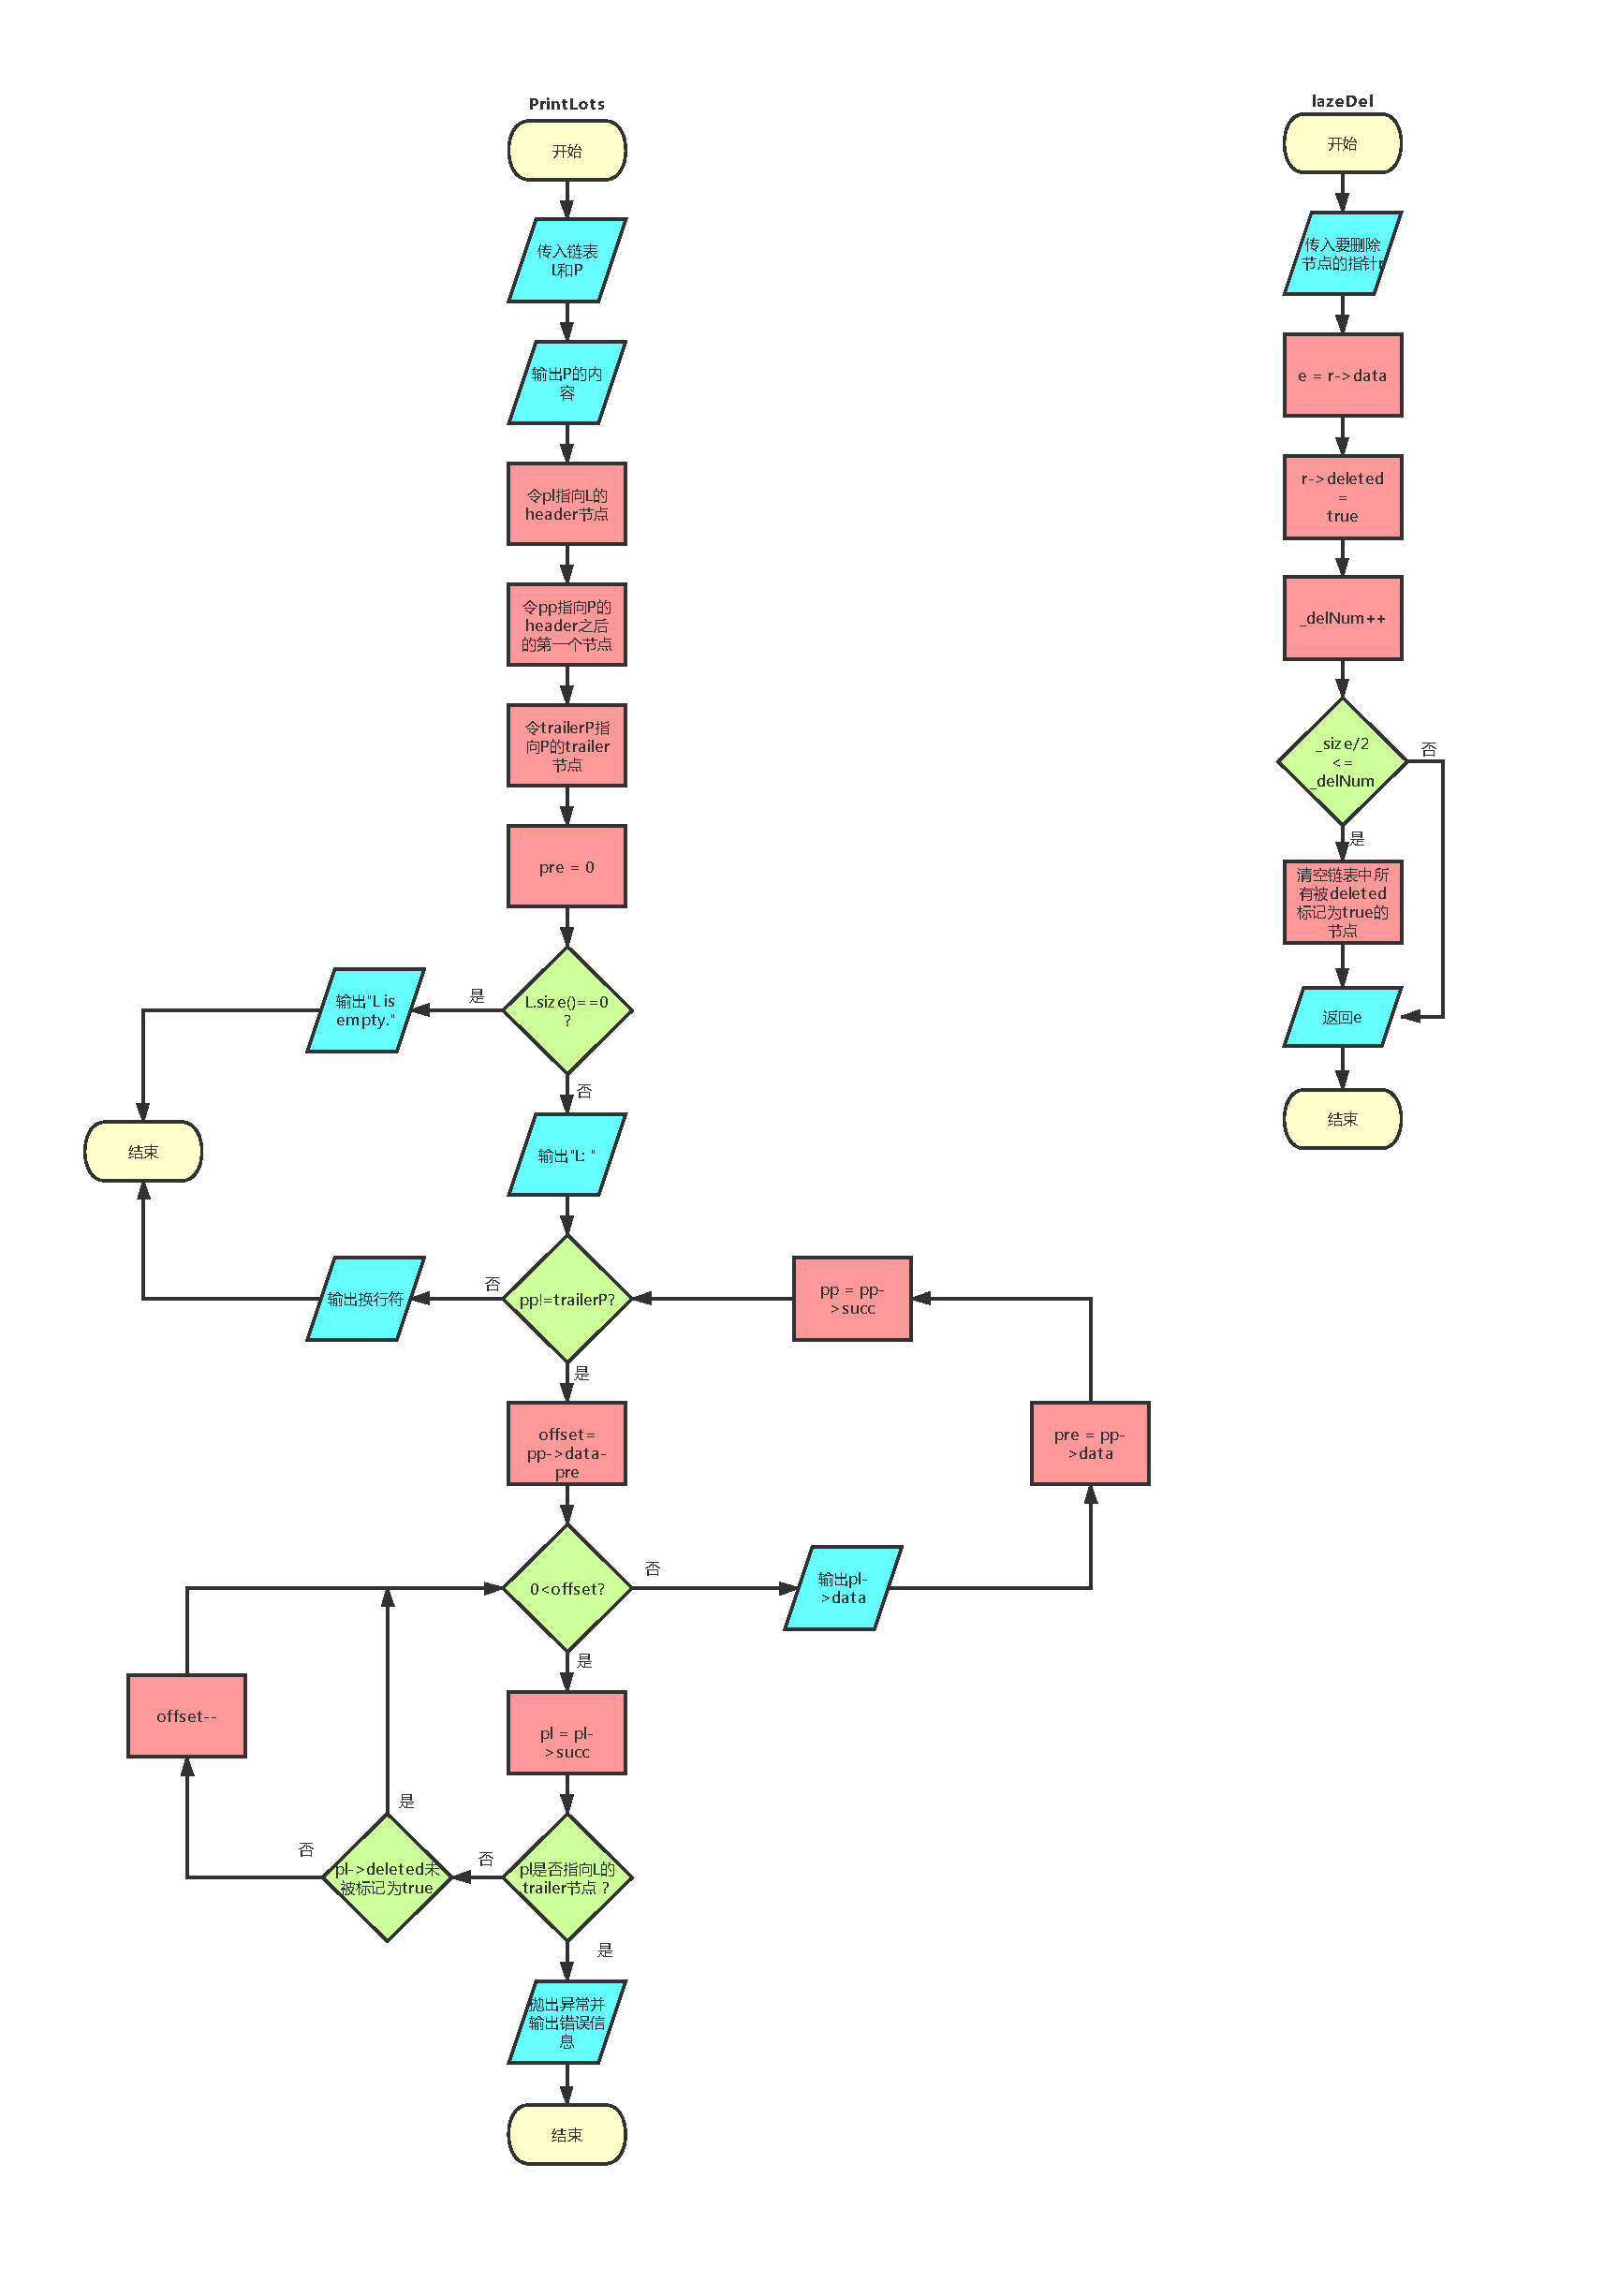
\includegraphics[width=20cm, height=25cm]{list_ADT.pdf} 
	\caption{$PrintLots$和$lazeDel$函数流程图} 
	\label{PrintsLots_and_lazeDel}
\end{figure}



\begin{figure}[H]
	\centering 
	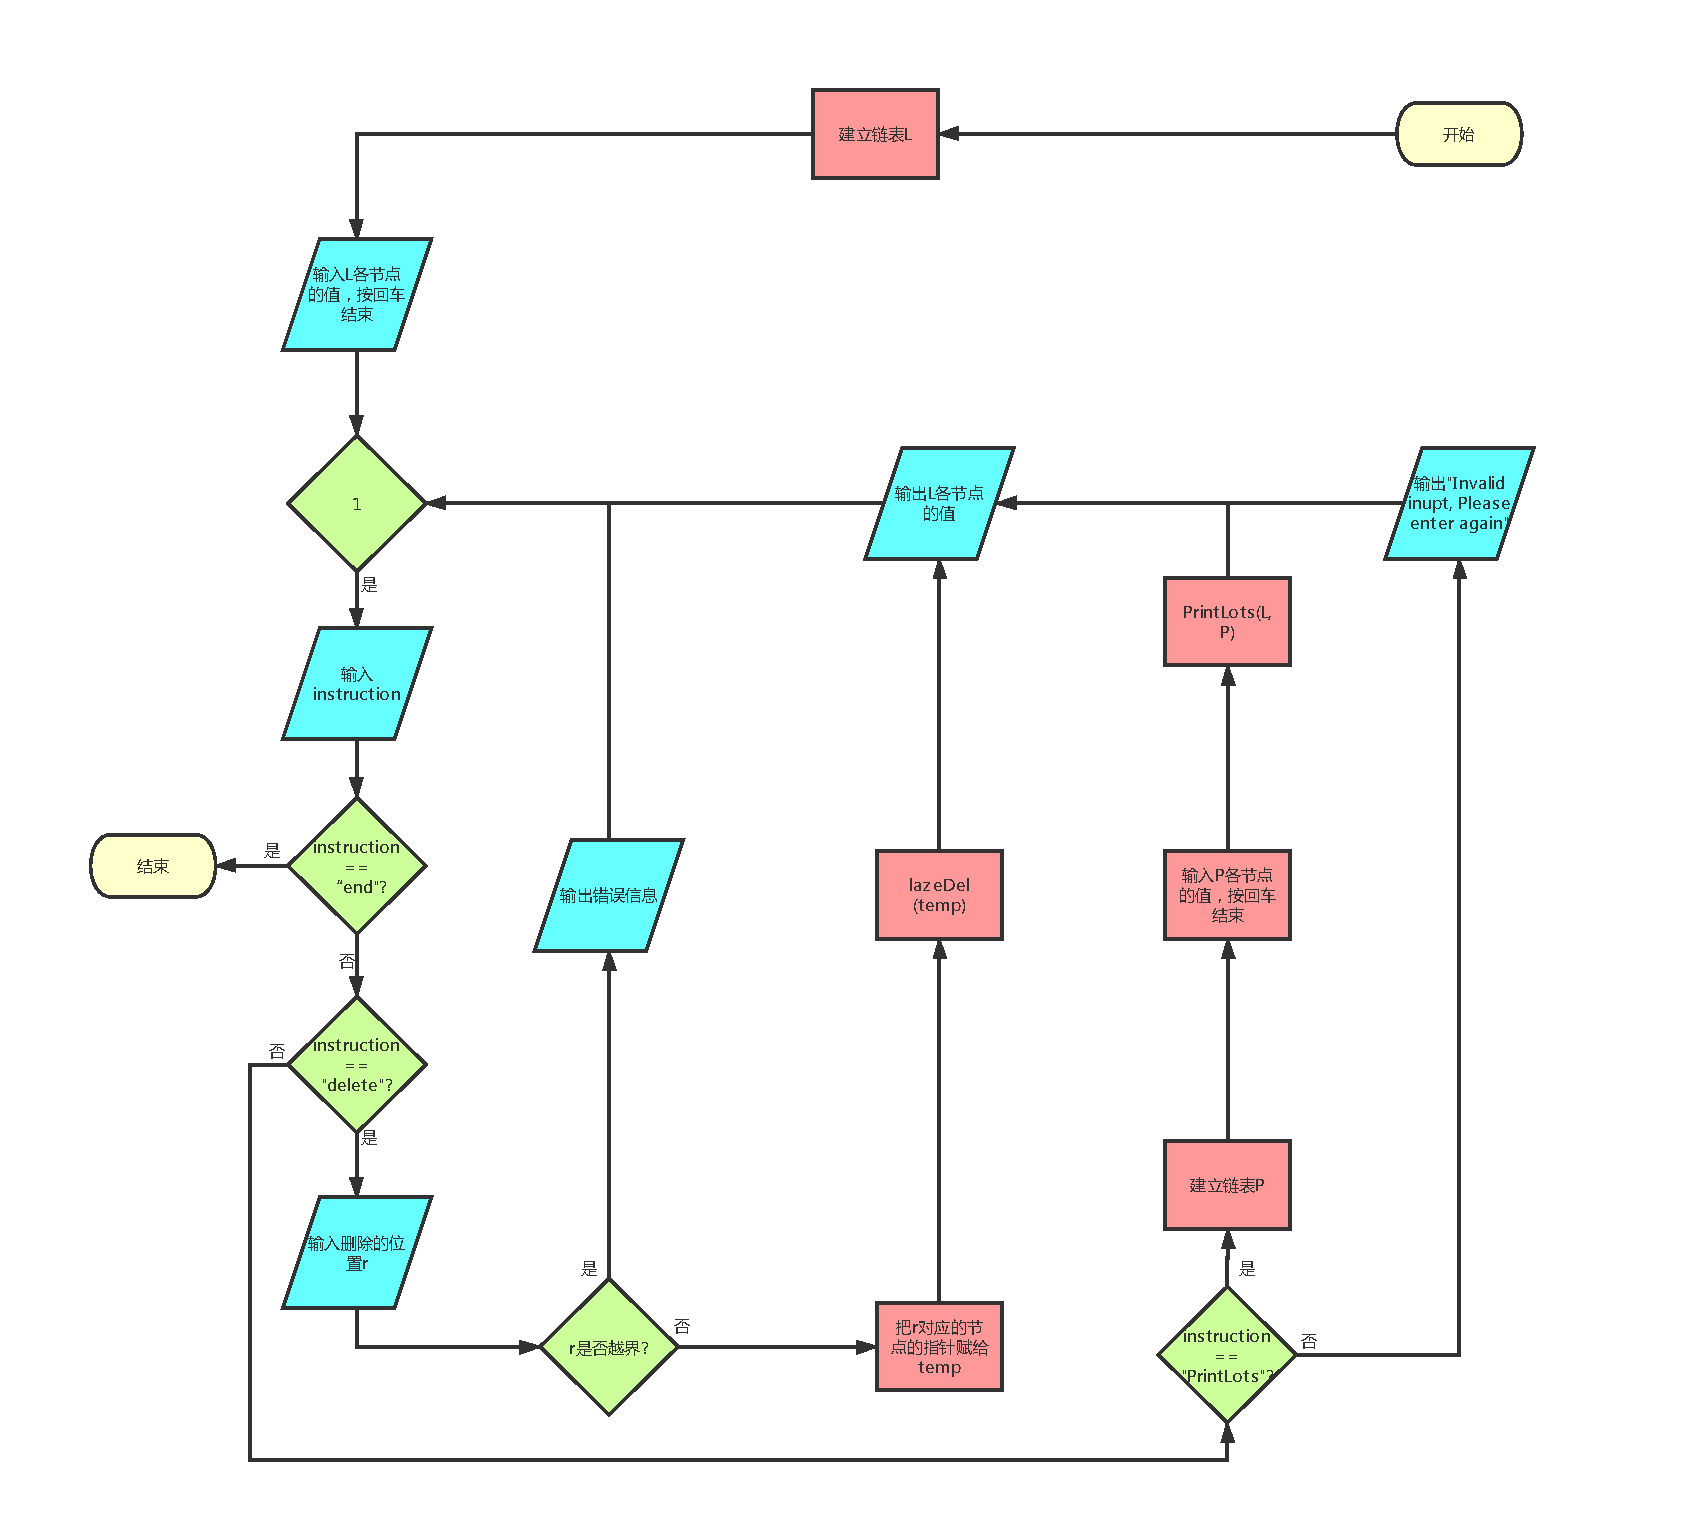
\includegraphics[width=20cm, height=23cm]{list_ADT_main.pdf} 
	\caption{$main$函数流程图} 
	\label{main}
\end{figure}
\newpage



	\section{编程实现}

	\begin{lstlisting}[language=C++,caption={list\_ADT代码},label={vec_code}]
#include<iostream>
#include<exception>
#include<stdexcept>
using namespace std;

template <typename T> 
class Node
{
    public:
        // member variables
        T data;
        Node<T>* pred;
        Node<T>* succ;
        bool deleted;
        // constructors
        Node() : data(0), pred(NULL), succ(NULL){}
        Node(T e, Node<T>* p=NULL, Node<T>* s=NULL) : data(e), pred(p), succ(s), deleted(false) {}
        // operation interface
        //Node<T>* insertAsPred(T const& e);
        //Node<T>* insertAsSucc(T const& e);
};


template <typename T> 
class List
{
    private:
        int _size;
        Node<T>* header;
        Node<T>* trailer;
        int _delNum;
    public:
        // constructors
        List();

        // destructor
        ~List();

        // operation interfaces
        Node<T>* insert(Node<T>* r, T const& e);// insert as pred
        void push_back(T e) {insert(trailer, e);}
        Node<T>* remove(Node<T>* r);
        int clear();
        void clear_mark();
        T lazeDel(Node<T>* r);
        Node<T>* getP(int r);
        void print();
        Node<T>* getHeader() {return header;}
        Node<T>* getTrailer() {return trailer;}
        int size() {return _size;}
};
// implement the functions of the List
template <typename T>
List<T>::List()
{
    header = new Node<T>;
    trailer = new Node<T>;
    header->succ = trailer;
    header->pred = NULL;
    trailer->pred = header;
    trailer->succ = NULL;
    _size = 0;
    _delNum = 0;
}

template <typename T>
Node<T>* List<T>::insert(Node<T>* r, T const& e)
{
    // insert as pred
    Node<T>* x = new Node<T>(e, r->pred, r);
    r->pred->succ = x;
    r->pred = x;
    _size++;
    return x;
}

template <typename T>
Node<T>* List<T>::remove(Node<T>* r)
{
    r->pred->succ = r->succ;
    r->succ->pred = r->pred;
    Node<T>* p = r->succ;
    delete r;
    _size--;
    if (r->deleted) _delNum--;
    return p;
}

template <typename T>
int List<T>::clear()
{
    int oldSize = _size;
    while(0 < _size)
        remove(header->succ);
    return oldSize;
}

template <typename T>
void List<T>::clear_mark()
{
    Node<T>* p = header->succ;
    while (p != trailer)
    {
        if (p->deleted)
            p = remove(p);
        else
            p = p->succ;
    }
    _delNum = 0;
    cout << "remove all nodes marked." << endl;
}

template <typename T>
List<T>::~List()
{
    clear();
    delete header;
    delete trailer;
}

template <typename T>
T List<T>::lazeDel(Node<T>* r)
{
    T e = r->data;
    r->deleted = true;
    _delNum++;
    if (_size/2 <= _delNum)
        clear_mark();
    return e;
}

template <typename T>
Node<T>* List<T>::getP(int r)
{
    Node<T>* p = header;
    while (0 < r)
    {
        p = p->succ;
        if (!p->deleted)
            r--;
        if (p == trailer)
            throw out_of_range("Overflow!");

    }

    return p;
}

template <typename T>
void List<T>::print()
{
    if (_size == 0)
    {
        cout << "The list is empty." << endl;
        return;
    }
    Node<T>* p = header;
    while ((p = p->succ) != trailer)
        if (!p->deleted)
            cout << p->data << " ";
    cout << endl;
}




// implement PrintLots
template <typename T>
void PrintLots(List<T>& L, List<T>& P)
{
    cout << "P: ";
    P.print();
    // pl points to the header of L 
    // and pp points to the first element of P
    Node<T>* pl = L.getP(0);
    Node<T>* pp = P.getP(1);
    Node<T>* trailerP = P.getTrailer();
    int pre = 0;
    if (!L.size())
    {
        cout << "L is empty." << endl;
        return;
    }
    cout << "L: ";
    while (pp != trailerP)
    {
        int offset = pp->data - pre;
        while (0 < offset)
        {
            pl = pl->succ;
            try
            {
                if (pl == L.getTrailer())
                    throw out_of_range("Overflow!");
            }catch(out_of_range &e)
            {
                cerr << endl << "Index " << pp->data <<" is out of range. " << e.what() << endl;
                return;
            }
            if (!pl->deleted)
                offset--;
        }
        cout << pl->data << " ";
        pre = pp->data;
        pp = pp->succ;
    }
    cout << endl;
}




int main()
{
    cout << "姓名:鲁国锐" << endl;
    cout << "学号:17020021031" << endl;
    cout << endl;
    cout << "instructions:" << endl;
    cout << "delete: 后跟一数字,执行懒惰删除操作" << endl;
    cout << "PrintLots: 后跟若干数字,务以空格分隔,以回车结束输入,为链表P的节点值,执行PrintLots操作" << endl;
    cout << "end: 结束程序" << endl;

    cout << endl << "请输入L中各节点的值,务必以空格分隔,以回车结束输入:" << endl;

    List<int> L;

    while (1)
    {
        int data;
        char c;
        cin >> data;
        cin.get(c);
        L.push_back(data);
        if (c == '\n')
            break;
    }
  
    while(1)
    {
        string instruction;
        cin >> instruction;
        if (instruction == "end")
            break;
        else if (instruction == "delete")
        {
            int r;
            cin >> r;
            Node<int>* temp;
            try
            {
                temp = L.getP(r);
            }catch(out_of_range &e)
            {
                cerr << "Index " << r << " is out of range. " << e.what() << endl;
                continue;
            }
            L.lazeDel(temp);
        }
        else if (instruction == "PrintLots")
        {
            List<int> P;
            while (1)
            {
                int data;
                char c;
                cin >> data;
                cin.get(c);
                P.push_back(data);
                if (c == '\n')
                    break;
            }
            PrintLots(L, P);
        }
        else
        {
            cout << "Invalide input, please enter again." << endl;
            continue;
        }
        

        L.print();
    }
}
	\end{lstlisting}
	
	\section{结果分析}
	
\begin{figure}[H]
	\centering 
	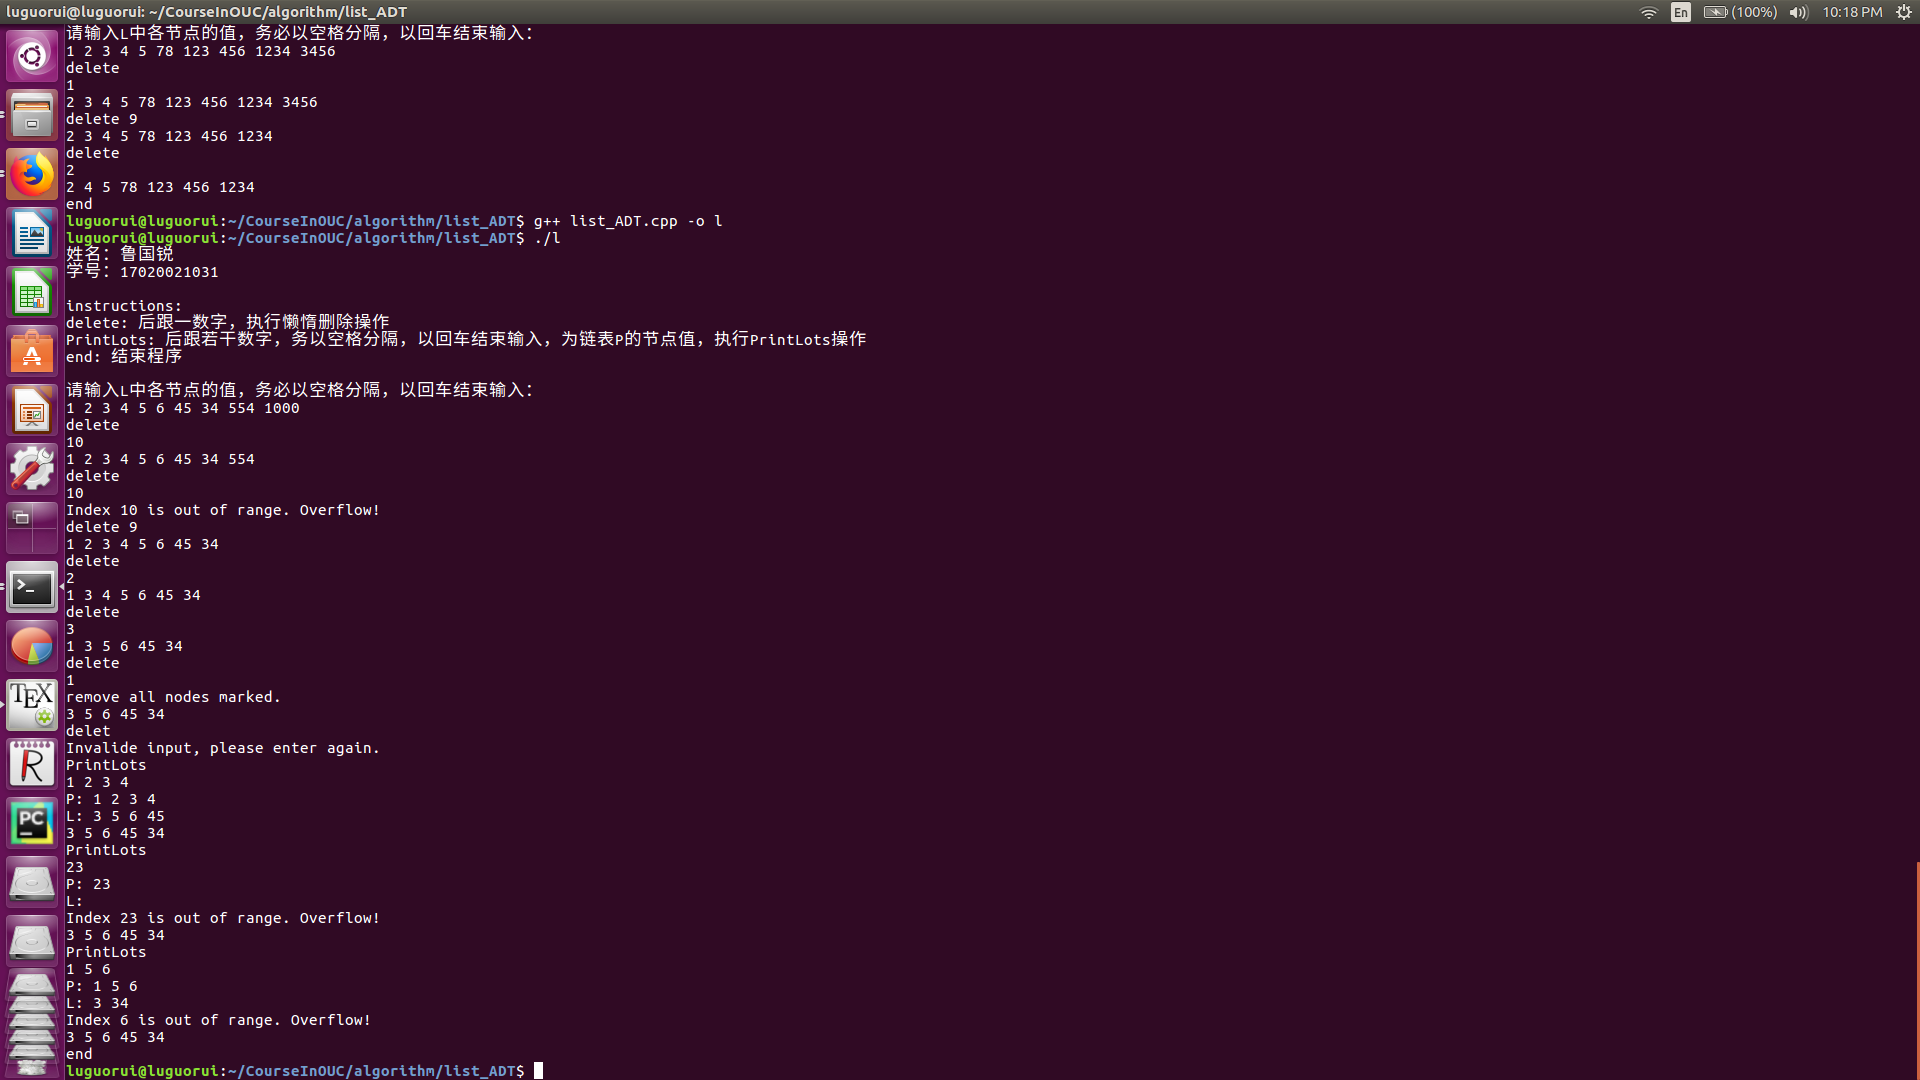
\includegraphics[width=18cm, height=23cm]{list_res.png} 
	\caption{结果} 
	\label{res}
\end{figure}
\newpage

	
	\section{总结体会}
	\indent 第一次做这道题时我是用$list$做的,因为一开始觉得$list$删除元素只需常数时间。但在实现过程中发现$list$在无法像$vector$那样在常数时间内访问任意一个元素,只能通过迭代器一个一个往后找,所以到最后两种实现方式的时间复杂度应该相差不多。但用$list$实现由于大量操作都是通过迭代器来实现的且迭代器之间不能进行算数操作,这使得它实现起来要更为复杂一些。

\bibliography{ref.bib}
\end{document}